%%%%%%%% ICML 2026 PLURALISTIC ALIGNMENT WORKSHOP SUBMISSION %%%%%%%%%%%%%%%%%

\documentclass{article}

\usepackage{microtype}
\usepackage{graphicx}
\usepackage{subcaption}
\usepackage{booktabs}
\usepackage{hyperref}
\usepackage[textsize=tiny]{todonotes}

\newcommand{\theHalgorithm}{\arabic{algorithm}}

\usepackage{icml2026}

\usepackage{amsmath}
\usepackage{amssymb}
\usepackage{mathtools}
\usepackage{amsthm}

\usepackage[capitalize,noabbrev]{cleveref}

\icmltitlerunning{Whose Alignment? Process Alignment Across Organizational Contexts}

\begin{document}

\twocolumn[
  \icmltitle{Whose Alignment? Measuring LLM Process Alignment\\
    Across Diverse Organizational Decision Contexts}

  \begin{icmlauthorlist}
    \icmlauthor{Anonymous Author 1}{anon}
    \icmlauthor{Anonymous Author 2}{anon}
  \end{icmlauthorlist}

  \icmlaffiliation{anon}{Anonymous Institution}

  \icmlkeywords{pluralistic alignment, LLM alignment, decision-making, Brunswik lens model, cue utilization, organizational alignment}

  \vskip 0.3in
]

\printAffiliationsAndNotice{}

% ── ABSTRACT ──────────────────────────────────────────────────────────────────

\begin{abstract}
Aligning AI systems with organizational decision-making is typically framed as a single-target problem: make the model behave like \emph{the} organization. We argue this framing obscures a deeper pluralistic challenge. We introduce the Contextualized Alignment Lens Model (CALM), which measures \emph{process alignment}: whether an LLM weights information as the organization does, not merely whether it reaches the same conclusions. Applying CALM to ECHR Article~6 decisions, process alignment strongly predicts output accuracy ($r = 0.85$, $p < .001$) and externalization substantially improves alignment for poorly-aligned models. Applying the same method to German consumer credit decisions, this relationship collapses ($r = 0.15$, $p = .60$): interventions produce inconsistent effects and the benchmark encodes potentially discriminatory historical patterns. This contrast is itself a pluralistic alignment finding: in contested domains, high process alignment is neither achievable via externalization nor unconditionally desirable. Output agreement alone cannot distinguish a model that has internalized an organizational policy from one that merely approximates its outcomes—process-level measurement is a necessary component of any pluralistic alignment evaluation.
\end{abstract}

% ── 1. INTRODUCTION ───────────────────────────────────────────────────────────

\section{Introduction}

Pluralistic alignment asks how AI systems can faithfully serve stakeholders with diverse, conflicting values rather than converging on a single dominant worldview \citep{sorensen2024roadmap}. Most work in this space focuses on \emph{between-person} plurality: aggregating individual preferences, handling annotation disagreements, or enabling models to adopt different user perspectives. We argue that \emph{between-organization} plurality is an equally important but largely neglected dimension. Organizations are distinct value-encoding institutions: they encode historically contingent decision policies that differ systematically across institutions, domains, and time. Models vary in which organizational value systems they implicitly align with, and this variation is not captured by any existing pluralistic alignment evaluation framework. Recognizing between-organization plurality expands the scope of pluralistic alignment from \emph{whose individual preferences?} to \emph{whose institutional norms?} This question has direct consequences for how AI systems are deployed, audited, and governed in high-stakes settings.

Organizations are not neutral information processors. They are repositories of knowledge accumulated through experience, culture, and institutional history \citep{nonaka1994dynamic}. Some of this knowledge is explicit: rules, policies, codified procedures. Much is tacit: embedded in practice and professional judgment, resistant to full articulation \citep{polanyi1966tacit,pakarinen2023relational}. When organizations deploy LLMs to replicate their decisions, they implicitly assume they can transfer this knowledge to a model. The tacit dimension resists this transfer.

This creates a problem distinct from output accuracy. An LLM can reach the right decision for the wrong reasons, weighting information differently than the organization while still achieving adequate accuracy on the observed distribution. We call this divergence the \emph{knowledge gap}: a mismatch between organizational and LLM cue-utilization policies that output agreement fails to detect \citep{geirhos2020shortcut,lebovitz2021ai}. The knowledge gap matters for process legitimacy \citep{tyler1988psychology}, generalization to novel cases, and the trustworthiness of AI-assisted decisions in regulated domains.

We present the Contextualized Alignment Lens Model (CALM), which operationalizes and measures this gap. CALM applies the Brunswikian lens model \citep{brunswik1952conceptual,hammond1964psychology} to estimate the cue-weighting policy of both organizations and LLMs from observed decisions, then computes cosine similarity between these policy vectors as the primary alignment metric. We test CALM in two domains:

\textbf{Study 1 (ECHR):} We analyze 1,000 ECHR Article~6 decisions across ten LLM models under three prompting conditions. We find sharp variation in baseline process alignment and show that explicit knowledge externalization substantially improves alignment for poorly-aligned models.

\textbf{Study 2 (German Credit):} We replicate CALM in consumer credit using the German Credit Dataset \citep{hofmann1994statlog}. Unlike the legal domain, the credit benchmark is derived from historical decisions that encode potentially discriminatory patterns. We find that alignment and accuracy are orthogonal, that externalization fails to reliably improve alignment, and that at least one model catastrophically over-corrects to base-rate feedback. This is a distinctively pluralistic challenge: \emph{whose values} should the model align to?

Together, these studies demonstrate a core thesis: CALM measures whether an LLM aligns with an organizational decision policy, but whether higher alignment is actually desirable depends on whether that policy itself encodes legitimate values. This is a distinctively pluralistic challenge that output-level evaluation cannot surface. Both studies also raise a third open question: whether a model's stated reasoning faithfully reflects its behavioral policy. CALM measures behavioral policy from observed decisions; whether a model's chain-of-thought tracks or diverges from that inferred policy remains an open challenge we address in the future work section.

% ── 2. BACKGROUND ─────────────────────────────────────────────────────────────

\section{Background}

\subsection{The Brunswik Lens Model}

The lens model \citep{brunswik1952conceptual,hammond1964psychology} represents judgment as a linear combination of observable cues: $J = \beta_0 + \sum_i \beta_i C_i$, where $C_i$ are cues and $\beta_i$ are learned weights. Applied to human decision-makers, it separates ecological validity (do cues genuinely predict outcomes?) from achievement (do the decision-maker's weights match ecological realities?). Applied to organizations and LLMs, it reveals whether they weight the same cues in the same direction and magnitude; that is, whether their \emph{observed behavioral policies} are aligned. Meta-analytic evidence confirms that human judges systematically misweight cues relative to ecological validities \citep{karelaia2008minds}; the same divergence between stated and behavioral weights appears when comparing organizational guidelines to individual practitioners' actual decisions \citep{smith2003factors}.

We estimate behavioral policies using ridge-regularized logistic regression on observed decisions, fitting identical cue sets to both the organizational benchmark and each LLM. The resulting coefficient vectors $\boldsymbol{\beta}$ represent each decision-maker's inferred cue-utilization policy. Alignment is measured as:
\begin{equation}
  \text{cos}(\theta) = \frac{\boldsymbol{\beta}_{\text{org}} \cdot \boldsymbol{\beta}_{\text{LLM}}}{\|\boldsymbol{\beta}_{\text{org}}\| \|\boldsymbol{\beta}_{\text{LLM}}\|}
\end{equation}

This metric is scale-invariant, symmetric, and bounded in $[-1, 1]$, where 1.0 indicates perfect alignment, 0 orthogonality, and negative values opposition.

\subsection{Pluralistic Alignment}

\citet{sorensen2024roadmap} distinguish three modes of pluralistic alignment: Overton pluralism (presenting a range of reasonable responses), distributional pluralism (reflecting population-level value distributions), and steerable pluralism (faithfully adopting a specified perspective when directed). The dominant approach to alignment via reinforcement learning from human feedback \citep{ouyang2022training} tends toward distributional consensus, encoding an aggregate value system rather than supporting genuine institutional plurality \citep{gabriel2020artificial}. CALM's externalization conditions are instances of steerable pluralism at the organizational level. This framing requires that steering be \emph{faithful}: the model must genuinely adopt the target policy, not merely mimic its surface outputs. CALM operationalizes this criterion by measuring whether the model's cue-weighting policy shifts toward the target organization's policy under externalization.

Prior work has shown that LLMs can solve judgment tasks at human-level accuracy while weighting information differently \citep{binz2023using}, and that output accuracy alone is insufficient for evaluating AI alignment in organizational settings \citep{wieringa2021means,lebovitz2021ai}. Our empirical results reinforce this: across both domains, models with very different process alignment scores achieve similar output accuracy, meaning that output-level evaluation systematically obscures which organizational values a model is actually implementing. Process-level measurement is therefore a necessary component of pluralistic alignment evaluation, not merely a supplementary one, particularly in high-stakes organizational deployment contexts.

% ── 3. THE CALM FRAMEWORK ─────────────────────────────────────────────────────

\section{The CALM Framework}

CALM measures process alignment between an organizational benchmark and LLM decision-making across three conditions:

\textbf{Baseline:} The model receives a structured case profile and decides without additional guidance. This reveals the model's \emph{implicit} cue-utilization policy, reflecting what it has learned through pretraining.

\textbf{Org-externalized:} The model receives the organization's cue-weighting policy, derived from ridge logistic regression on the organization's historical decisions, as explicit guidance before the case. High-weighted cues are described as strong indicators; medium-weighted cues as moderate; low-weighted cues as weak. This tests whether making the tacit explicit closes the knowledge gap.

\textbf{Introspective-externalized:} The model is shown how its own baseline cue-weighting policy diverges from the organization's (aggregate patterns across all cases) and instructed to self-correct. This tests whether self-directed adjustment can supplement or replace explicit guidance.

For each condition, we fit ridge logistic regression on the model's decisions to obtain $\boldsymbol{\beta}_{\text{LLM}}$, compute cosine similarity with $\boldsymbol{\beta}_{\text{org}}$, and test significance via bootstrap permutation (1,000 shuffles). Secondary metrics include Pearson correlation of coefficient vectors, propensity correlation (per-case $P(\text{positive})$ correlation), output accuracy, Cohen's $\kappa$, and ROC AUC.

CALM thus serves two functions depending on the domain. Where the organizational benchmark reflects a legitimate, well-specified normative policy, CALM is a \emph{calibration} tool: it quantifies policy divergence and guides externalization to close the gap. Where the benchmark encodes historically contested practices—decision policies that conflict with contemporary legal or ethical standards—CALM is an \emph{audit} tool: it renders the behavioral policy legible so that its normative implications can be examined rather than assumed. The two studies below are designed as deliberate tests of each function.

% ── 4. STUDY 1: ECHR ──────────────────────────────────────────────────────────

\section{Study 1: ECHR Article 6 Decisions}

\subsection{Context and Data}

We analyze 1,000 ECHR Article~6 decisions (50\% violation / 50\% no violation). Cues were coded as 45 binary features organized into nine families (Delay, Counsel, EvidenceAndArms, TribunalIntegrity, etc.) using GPT-5.4-mini with a codebook derived from Article~6 jurisprudence. We note a potential conflict of interest: GPT-5.4-mini serves as both the cue-coding instrument and one of the ten test models. To mitigate circularity, cue coding was performed under a fixed, pre-specified codebook with no access to model decisions, and a 10\% random sample of coded cases was verified by manual review, yielding agreement above 90\%. We tested ten models selected to span sizes, providers, and geographical origin: GPT-5.4, GPT-5.4-mini, GPT-5.4-nano, Grok 4.1 Fast, Claude Haiku 4.5, Gemma 4 (31B), Minimax M2.7, Mistral Large, DeepSeek-v3.2, and Qwen 3.6 Plus, spanning US-, European-, and China-based providers.

The court's ridge logistic regression achieves ROC AUC = 0.714, confirming that binary cues capture meaningful but partial variance in judicial reasoning. The most heavily weighted cue families are EvidenceAndArms and Delay, consistent with prior computational studies of ECHR outcomes \citep{aletras2016predicting,chalkidis2021paragraph}.

\subsection{Baseline Process Alignment}

Baseline process alignment varies widely across the ten models. Cosine similarity ranges from $-0.211$ (GPT-5.4-nano) to $+0.844$ (GPT-5.4-mini). Three models cluster above $r_{\cos} = 0.82$: GPT-5.4-mini (0.844), Grok 4.1 Fast (0.842), and GPT-5.4 (0.824). Three others show moderate positive alignment: Qwen 3.6 Plus (0.750), Gemma 4 (31B) (0.710), and Minimax M2.7 (0.592). Four models fall near zero or below: Mistral Large (0.083), DeepSeek-v3.2 (0.062), Claude Haiku 4.5 ($-0.057$), and GPT-5.4-nano ($-0.211$). This spread does not track general-purpose benchmark performance or pricing tier.

This variation reveals implicit value plurality: models trained on similar data encode systematically different cue-weighting policies. Claude Haiku 4.5 illustrates the output-process paradox: its policy vector is orthogonal to the court's ($r_{\cos} = -0.057$) while its discriminative AUC (0.797) exceeds that of GPT-5.4-mini (0.770), yet it reaches comparable discriminative ability via an entirely different reasoning path. Across all 30 model--condition pairs, Pearson $r = 0.85$ ($p < .001$) between cosine similarity and output accuracy confirms that process alignment is the dominant predictor of performance in this domain (see Figure~\ref{fig:scatter}, left panel).

\subsection{Effect of Externalization}

Org-externalization moves the cosine estimate in the predicted direction for 8 of 10 models, producing statistically significant gains (one-sided $p < .05$) for three initially misaligned models: GPT-5.4-nano ($\Delta = +0.906$), Claude Haiku 4.5 ($\Delta = +0.682$), and Minimax M2.7 ($\Delta = +0.176$). Ceiling effects appear for models already well-aligned: GPT-5.4-mini ($\Delta = +0.045$, n.s.) and GPT-5.4 ($\Delta = +0.045$, n.s.), consistent with the hypothesis that externalization has little room to improve a model whose implicit policy already matches the organization's. Introspective externalization moves the point estimate in the predicted direction for 6 of 10 models; comparable gains appear for Claude Haiku 4.5 ($\Delta = +0.755$), but Grok 4.1 Fast regresses sharply ($\Delta = -0.346$, $p = .002$ in the worsening direction), its well-calibrated implicit policy disrupted by self-correction feedback.

% ── 5. STUDY 2: GERMAN CREDIT ─────────────────────────────────────────────────

\section{Study 2: German Credit Decisions}

\subsection{Context and the Fairness Tension}

The German Credit Dataset \citep{hofmann1994statlog} contains 1,000 consumer credit decisions by a German bank, with a 70\% Good / 30\% Bad base rate and 20 cues including numerical (loan duration, credit amount, age) and categorical (credit history, employment status, housing) attributes.

This domain introduces a tension absent from the ECHR study. Several cues are protected attributes under contemporary anti-discrimination law: \texttt{personal\_status\_sex}, \texttt{age\_years}, and \texttt{foreign\_worker}. The organizational normative model is derived from historical human decisions that may encode discriminatory patterns. The original credit officers may have weighted these attributes in ways that disadvantaged women, older applicants, or foreign workers. High process alignment with this benchmark is therefore not unconditionally desirable \citep{selbst2019fairness,dolata2022sociotechnical}. A model achieving $r_{\cos} \approx 1.0$ with the normative model may be faithfully reproducing institutional discrimination.

This surfaces a core pluralistic alignment question: whose values should the model align to? The organization's historically documented decision policy? Its stated ethical commitments? Contemporary regulatory standards? These targets may conflict, and CALM makes this conflict visible precisely because it measures the \emph{actual} weighting policy rather than stated intent.

\subsection{Setup}

We apply five LLMs (Claude Haiku 4.5, GPT-5.4-mini, GPT-5.4-nano, Grok 4.1 Fast, DeepSeek-v3.2) under three conditions to all 1,000 cases. These five were selected to span the range of baseline alignment observed in Study 1, from strongly positive ($r_{\cos} > 0.5$) to negative, while limiting the computational cost of running all three conditions across 1,000 cases in this replication study; the remaining Study 1 models will be included in a full replication. To address the original dataset's class imbalance (70/30), we evaluate on a balanced held-out subset of 600 cases (300 Good, 300 Bad; stratified random sample, seed = 42) for all comparisons. The normative logistic regression on this subset achieves 75.1\% accuracy and ROC AUC = 0.751, establishing the performance ceiling.

The org-externalized condition injects normative cue weights (derived from ridge logistic regression on the full 1,000-case dataset) as bank policy before each case, structured by tier (strong, moderate, weak) with direction. The introspective condition provides each model with a personalized deviation profile: which cues it over- and under-weighted in the baseline condition relative to the normative model.

\begin{figure*}[t]
  \centering
  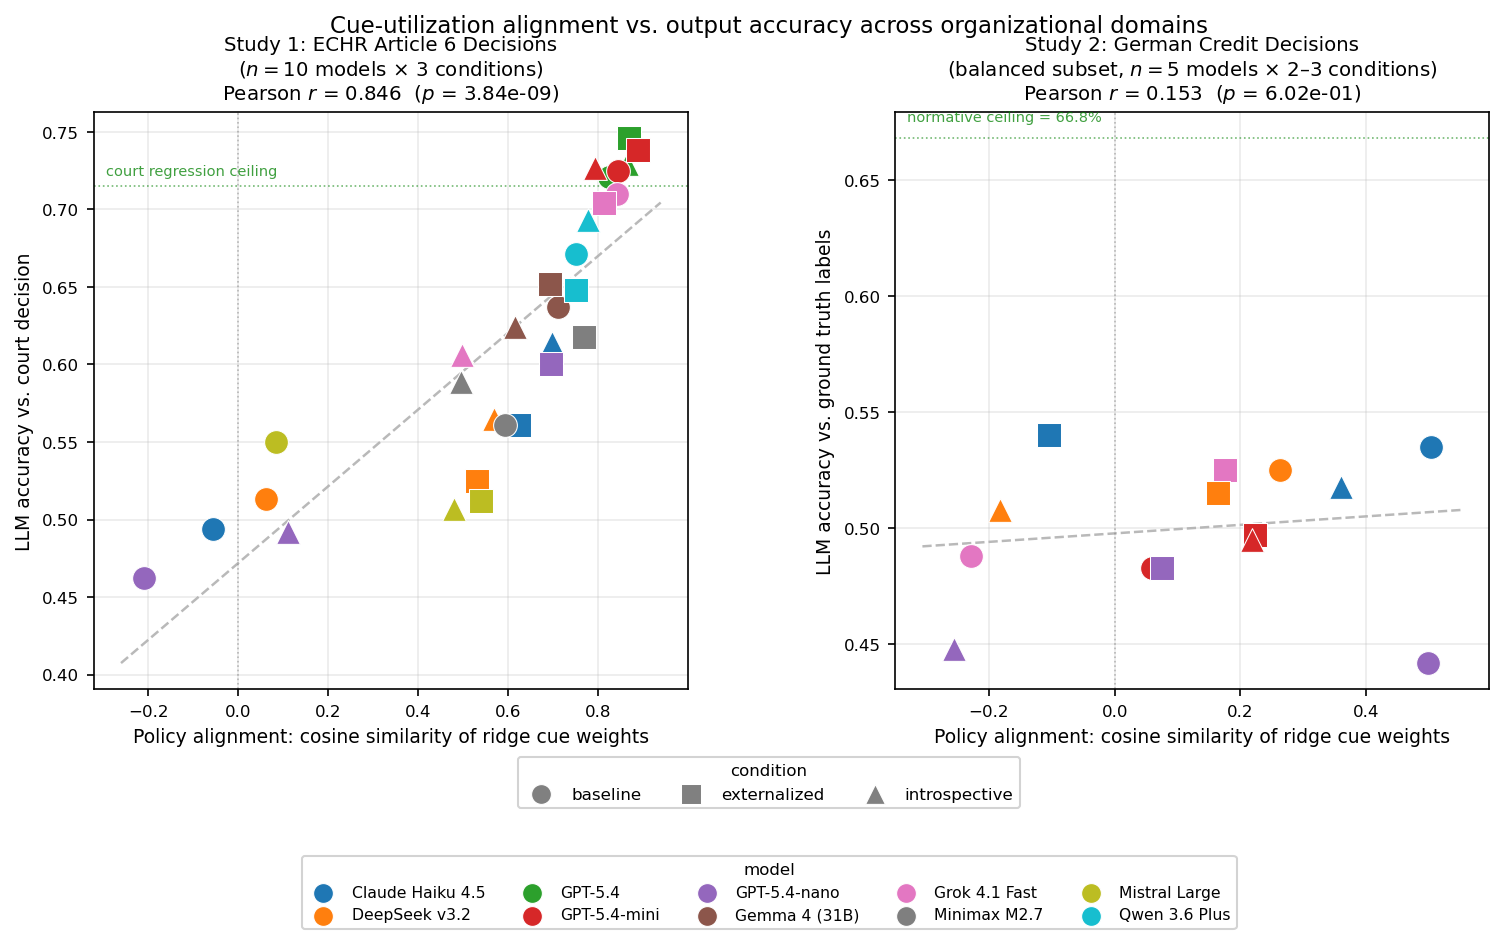
\includegraphics[width=\textwidth]{figures/alignment_vs_accuracy_comparison.png}
  \caption{Policy alignment (cosine similarity) vs.\ output accuracy across both domains. \textbf{Left:} ECHR Article~6 decisions show a strong positive relationship ($r = 0.85$, $p < .001$, $n = 10$ models $\times$ 3 conditions); the dotted line marks the court regression ceiling. \textbf{Right:} German Credit decisions (balanced subset) show a flat, non-significant relationship ($r = 0.15$, $p = .60$, $n = 5$ models $\times$ 2--3 conditions); the dotted line marks the normative ceiling (75.1\%). The contrast is the central finding: in a domain with a contested normative benchmark, process alignment and output accuracy decouple completely.}
  \label{fig:scatter}
\end{figure*}

\subsection{Baseline Process Alignment}

Table~\ref{tab:german-baseline} reports baseline results. Cosine similarity varies across models (range: $-0.229$ to $+0.503$), indicating heterogeneous implicit policies comparable in spread to the ECHR domain.

This variation does not, however, translate into accuracy differences. All five models achieve 44--54\% accuracy on the balanced subset, leaving a substantial gap relative to the 75.1\% normative ceiling. More tellingly, across all balanced model--condition pairs, the Pearson correlation between cosine similarity and output accuracy is $r = 0.15$ ($p = .60$), effectively zero. This stands in sharp contrast to the ECHR domain ($r = 0.85$, $p < .001$). In the credit domain, process alignment and output accuracy are orthogonal: knowing how closely a model's policy resembles the historical benchmark tells us nothing about its classification performance.

\begin{table}[t]
  \caption{Baseline process alignment in the German Credit domain (balanced subset, $n=600$). Normative ceiling: 75.1\% accuracy, AUC = 0.751. Good\% = proportion of cases classified as Good risk.}
  \label{tab:german-baseline}
  \begin{center}
    \begin{small}
      \begin{tabular}{lcccc}
        \toprule
        Model & $r_{\cos}$ & Acc (\%) & AUC & Good\% \\
        \midrule
        Claude Haiku 4.5 & $+0.503$ & 53.5 & 0.930 &  9.2 \\
        GPT-5.4-mini     & $+0.060$ & 48.3 & 0.961 & 68.0 \\
        GPT-5.4-nano     & $+0.499$ & 44.2 & 0.936 & 50.5 \\
        Grok 4.1 Fast    & $-0.229$ & 48.8 & 0.882 & 37.5 \\
        DeepSeek-v3.2    & $+0.264$ & 52.5 & 0.925 &  5.5 \\
        \bottomrule
      \end{tabular}
    \end{small}
  \end{center}
\end{table}

The Good\% column reveals another anomaly: the implicit approval rates span 5.5\% (DeepSeek) to 68\% (GPT-5.4-mini), despite all models encountering the same balanced cases. DeepSeek and Claude Haiku classify almost all applicants as Bad risk; GPT-5.4-mini closely tracks the 70\% historical base rate. These are fundamentally different implicit policies about credit risk, yet they produce nearly identical accuracy figures.

\subsection{Effect of Externalization}

Table~\ref{tab:german-extern} reports alignment changes under both interventions. The pattern is inconsistent and, on average, negative.

\begin{table}[t]
  \caption{Change in process alignment under org-externalization and introspective-externalization ($\Delta r_{\cos}$, German Credit balanced subset). $^{\dag}$Grok introspective condition excluded: model classified 99.5\% of cases as Good (degenerate over-correction).}
  \label{tab:german-extern}
  \begin{center}
    \begin{small}
      \begin{tabular}{lcccc}
        \toprule
        & \multicolumn{2}{c}{Org-ext} & \multicolumn{2}{c}{Introspective} \\
        \cmidrule(lr){2-3}\cmidrule(lr){4-5}
        Model & $r_{\cos}$ & $\Delta$ & $r_{\cos}$ & $\Delta$ \\
        \midrule
        Claude Haiku 4.5 & $-0.104$ & $-0.607$ & $+0.360$ & $-0.143$ \\
        GPT-5.4-mini     & $+0.224$ & $+0.164$ & $+0.219$ & $+0.159$ \\
        GPT-5.4-nano     & $+0.076$ & $-0.423$ & $-0.256$ & $-0.755$ \\
        Grok 4.1 Fast    & $+0.176$ & $+0.405$ & — & $^{\dag}$ \\
        DeepSeek-v3.2    & $+0.164$ & $-0.100$ & $-0.183$ & $-0.447$ \\
        \bottomrule
      \end{tabular}
    \end{small}
  \end{center}
\end{table}

Org-externalization moves two models toward the normative policy (GPT-5.4-mini $\Delta = +0.164$; Grok $\Delta = +0.405$) and moves three away (Claude Haiku $\Delta = -0.607$; GPT-5.4-nano $\Delta = -0.423$; DeepSeek $\Delta = -0.100$). Claude Haiku's sharp negative shift is particularly notable: providing the explicit normative policy as guidance \emph{reduces} its alignment, suggesting that explicit credit scoring instructions push the model toward a different implicit reasoning pattern. Introspective externalization fares worse overall: three of four evaluable models decline in alignment ($\Delta$ range: $-0.755$ to $+0.159$).

\textbf{Grok's degenerate over-correction.} When given personalized deviation feedback noting its under-approval relative to the 70\% historical base rate, Grok 4.1 Fast classified 99.5\% of cases as Good risk in the introspective condition, effectively inverting its prior 37.5\% approval rate. Rather than recalibrating toward the normative policy, Grok 4.1 Fast treated the base-rate instruction as a decision rule. This over-correction renders cosine similarity analysis uninformative for this cell and illustrates a failure mode of introspective calibration: models may respond to statistical feedback with behavioral compliance rather than genuine policy adjustment.

\subsection{Protected Attribute Weighting}

Inspection of the descriptive tier analysis reveals that LLMs systematically diverge from the normative model on protected attributes. In the baseline condition, Claude Haiku weights \texttt{foreign\_worker} as HIGH in 56.8\% of cases, despite the normative model rating it LOW, while classifying \texttt{age\_years} and \texttt{personal\_status\_sex} as NOT\_MENTIONED in 34.5\% and 36.8\% of cases respectively, against a normative MEDIUM weighting for both. Interventions partially shift these patterns but do not consistently align them with the normative benchmark. This points to a deeper issue: models appear to possess domain knowledge about protected attributes, including awareness that these should not serve as decision criteria, which competes with and may override the organizational policy signal. Process alignment is thus doubly contested in this domain: models may resist adopting the organizational policy precisely on the cues where it diverges most from contemporary fairness norms.

% ── 6. CROSS-DOMAIN DISCUSSION ────────────────────────────────────────────────

\section{Discussion}

\subsection{The Contrast Is the Finding}

Our two studies produce a sharp cross-domain contrast. In the ECHR domain, process alignment predicts output accuracy strongly ($r = 0.85$), models start from diverse baselines, and externalization reliably closes the gap for misaligned models. In the German Credit domain, the alignment-accuracy relationship collapses ($r = 0.15$), LLMs achieve uniformly poor accuracy despite varied alignment (44--54\% against a 75.1\% ceiling), and interventions produce inconsistent results.

We argue this contrast reflects a fundamental difference in the nature of the two organizational benchmarks. The ECHR's cue-weighting policy reflects accumulated legal doctrine: there is a relatively stable, publicly articulated standard that well-trained models can learn from pretraining data and that externalization can reinforce. German consumer credit decisions in the 1990s reflect a combination of legitimate risk signals (loan duration, credit amount, repayment burden) and historically contingent social judgments that have since been partially superseded by anti-discrimination law.

The result is that high process alignment with the German Credit normative model is not a clean target. A model that perfectly replicates the historical credit officer's cue-weighting policy may be accurately capturing credit risk signals, or faithfully reproducing discriminatory judgments about gender, age, and immigration status. CALM cannot adjudicate this; its contribution is to make the behavioral policy legible so that the question can be asked.

A natural objection is that the two domains were selected to produce this contrast, rendering the contestedness explanation post hoc. We address this directly. The domains were chosen on the basis of data availability, institutional prominence, and structural distinctiveness before results were examined. The contestedness hypothesis carries genuine empirical content: it predicts that the alignment-accuracy relationship will be strong where the normative benchmark reflects stable, publicly-articulated standards, and weak where it reflects historically contingent social judgments. This prediction would be falsified if a domain with clearly contested norms showed a strong alignment-accuracy correlation, or if a domain with a legitimate normative benchmark showed the orthogonality observed in German Credit. Testing CALM on additional domains—clinical guidelines, hiring rubrics, audit standards—would allow norm stability and discriminative ceiling to be varied independently, providing a more rigorous test of the mechanism.

\subsection{Steerable Pluralism Requires Process-Level Measurement}

\citet{sorensen2024roadmap} argue that steerable pluralism is the most practically important mode of pluralistic alignment: systems should be steerable toward the perspective of a specified stakeholder when directed. Our externalization results demonstrate that this steerability is partial in the legal domain and largely absent in the credit domain. Residual divergence persists even with explicit policy guidance, consistent with the view that tacit organizational knowledge cannot be fully captured in a prompt \citep{polanyi1966tacit}.

Steerability is not, however, straightforwardly \emph{desirable} in the credit domain. An organization might specify its historical decision policy only to find that it encodes attributes that models resist using precisely because they violate training-time alignment guidelines. The tension between organizational process alignment and model-level safety alignment is a distinctively pluralistic challenge that output-level evaluation cannot surface.

\subsection{The Faithfulness Problem}

CALM infers cue-weighting policy from observed decisions, treating the model as a black box. It is worth emphasizing that this approach does not depend on chain-of-thought reliability. The estimated $\boldsymbol{\beta}_{\text{LLM}}$ captures the actual cue-weighting function the model implements across the full case set, derived from input-output pairs alone. This is the behavioral ground truth, independent of what the model claims to be doing in any individual reasoning trace. If anything, the potential divergence between stated reasoning and behavioral policy strengthens the case for CALM: a model can produce coherent, on-policy justifications while behaviorally weighting entirely different cues, meaning that auditing stated reasoning is insufficient and behavioral measurement is essential.

A separate but related question is whether a model's explicit chain-of-thought reasoning, produced when justifying a decision, reflects the same policy as its behavioral decisions. Prior work suggests systematic divergence: models can produce plausible-sounding reasoning that does not correspond to the features that actually drove their output \citep{lanham2023measuring,turpin2024language}. In the organizational alignment context, this creates a faithfulness problem with practical stakes. A model that explicitly cites the right cues in its reasoning while behaviorally weighting different ones would pass a surface-level audit but fail a process-alignment audit. Conversely, a model might weight cues in a normatively appropriate way while producing reasoning that references protected attributes.

A natural extension of the present work is to compare CALM's behavioral policy estimates against cue weights extracted from explicit LLM reasoning, for instance by asking a scoring model to classify which cues were mentioned as influential in each case, then regressing those mention rates against the same cue set. If behavioral policy and stated reasoning track each other, then explicit reasoning is a reliable proxy for process alignment. If they diverge, auditing stated reasoning is insufficient and behavioral measurement via CALM is essential. We leave this analysis to future work.

\subsection{Process Alignment as an Audit Tool}

Our findings suggest a revised framing for CALM. In domains with legitimate, well-specified normative benchmarks (like ECHR), CALM is a \emph{calibration} tool: it measures how far a model deviates from the target policy and guides externalization to close the gap. In domains with contested normative benchmarks (like German Credit), CALM is primarily an \emph{audit} tool: it surfaces which protected and non-protected attributes each model is weighting, how those weights compare to the historical benchmark, and how they shift under intervention. This diagnostic use does not require that the normative model be a legitimate alignment target; the comparison need only be informative.

For organizations deploying LLMs in high-stakes decision settings, CALM audits provide a third form of evaluation alongside output accuracy (are decisions correct?) and demographic disparity metrics (are decisions fair?): \emph{are decisions reached in the right way?} Process legitimacy is increasingly recognized as a legal and ethical requirement in consequential AI deployments \citep{tyler1988psychology}, and CALM provides a scalable method for measuring it from observed decisions.

\subsection{Policy Implications}

Our findings have direct relevance to emerging AI governance frameworks. The EU AI Act classifies consumer credit scoring as a high-risk AI application (Annex III), requiring conformity assessments, transparency obligations, and human oversight. Current regulatory guidance focuses primarily on output-level metrics: accuracy, demographic parity, and calibration. Our results suggest this is insufficient. Two systems with identical accuracy and disparity profiles can differ dramatically in \emph{how} they reach their decisions, with one replicating historically discriminatory weighting policies and the other not. CALM provides a process-level audit mechanism that can surface this divergence from observed decisions alone, without requiring access to model weights or internal representations.

More broadly, the question of \emph{whose} organizational policy an LLM should align with is itself a governance question. Organizations deploying AI in regulated domains must specify not just a performance target but a normative target: which version of their decision policy should serve as the alignment reference, whether historical practice, stated ethical commitments, or current regulatory standards. CALM makes this choice explicit and auditable. We argue that pluralistic alignment frameworks should engage directly with these governance questions, since the technical problem of measuring alignment cannot be separated from the normative problem of deciding what to align to \citep{russell2019human,gabriel2020artificial}.

% ── 7. CONCLUSION ─────────────────────────────────────────────────────────────

\section{Conclusion}

We have presented CALM and applied it across legal (ECHR) and financial (German Credit) domains. The results show that the relationship between process alignment and output accuracy is domain-dependent: strong and reliable where the organizational benchmark reflects stable, publicly-articulable norms; absent where it reflects historically contingent and contested values. In the credit domain, interventions that successfully shift model behavior in the legal domain fail to reliably improve alignment, and at least one model responds to statistical feedback with degenerate overcorrection. The credit domain also surfaces the fairness tension inherent in organizational alignment: models may actively resist adopting historical decision policies on protected attributes.

We conclude that organizational alignment is not a single problem. It requires asking: which organization, which policy, and from whose perspective? CALM provides a measurement framework for asking these questions empirically. We argue that pluralistic alignment research should extend beyond between-person value diversity to encompass between-organization diversity, the incommensurability of tacit institutional knowledge, and the ethical contestability of the norms that organizational benchmarks encode.

% ── IMPACT STATEMENT ──────────────────────────────────────────────────────────

\section*{Impact Statement}

This work develops methods for measuring whether AI systems reason as specific organizations do. These methods have positive applications in auditing AI decision-making for process legitimacy and fairness. The same methods could, in principle, be used to align AI systems with organizations whose decision policies are discriminatory or harmful. We argue that surfacing this risk, as CALM does in the German Credit analysis, is preferable to leaving it invisible in output-level evaluations.

% ── REFERENCES ────────────────────────────────────────────────────────────────

\bibliography{calm_references}
\bibliographystyle{icml2026}

\end{document}
